

\section{True/False Questions (10 pts)} 
For each question, please provide a short explanation to support your judgment.

\paragraph{Problem 1.1 (2 pts)} Even if there exist a set of weight for a Madaline model that can perfectly fulfill a learning task, there's no guarantee that this set of weight can be found if we train the Madaline model from a random initialization with the error correction (MD-II) rule. 

\paragraph{Problem 1.2 (2 pts)} The latency of a neural network measured on a specific processor is not always positively related to its theoretical FLOPS.

\paragraph{Problem 1.3 (2 pts)} Consider activation function $f(x) = \log(1 + \exp(x))$. The gradient of this function only vanish when $x \rightarrow  -\infty$, so it is easier to train compared to sigmoid, whose gradients vanish when $x \rightarrow$ both $-\infty$ and $+\infty$.

\paragraph{Problem 1.4 (2 pts)} On image recognition tasks, the convolution layers, compared to fully-connected layers, usually lead to better performance by exploiting shift invariant images features. 

\paragraph{Problem 1.5 (2 pts)} Consider two convolutional layers stacked together with a ReLU non-linearity in the middle. The first one has kernel size 5 and stride 2 and the second one has kernel size 3 stride 1. The combined receptive field of the stacked layers is 9.


\section{Adalines (15 pts)}

In the following problems, you will be asked to derive the output of a given Adaline, or propose proper weight values for the Adaline to mimic the functionality of some simple logic functions. For all problems, please consider $+1$ as \textbf{True} and $-1$ as \textbf{False} in the inputs and outputs.

\paragraph{Problem 2.1 (3 pts)} Observe the Adaline shown in Figure~\ref{fig:2.1}, fill in the feature $s$ and output $y$ for each pair of inputs given in the truth table. What logic function is this Adaline performing?

\begin{figure}[h]
\centering
  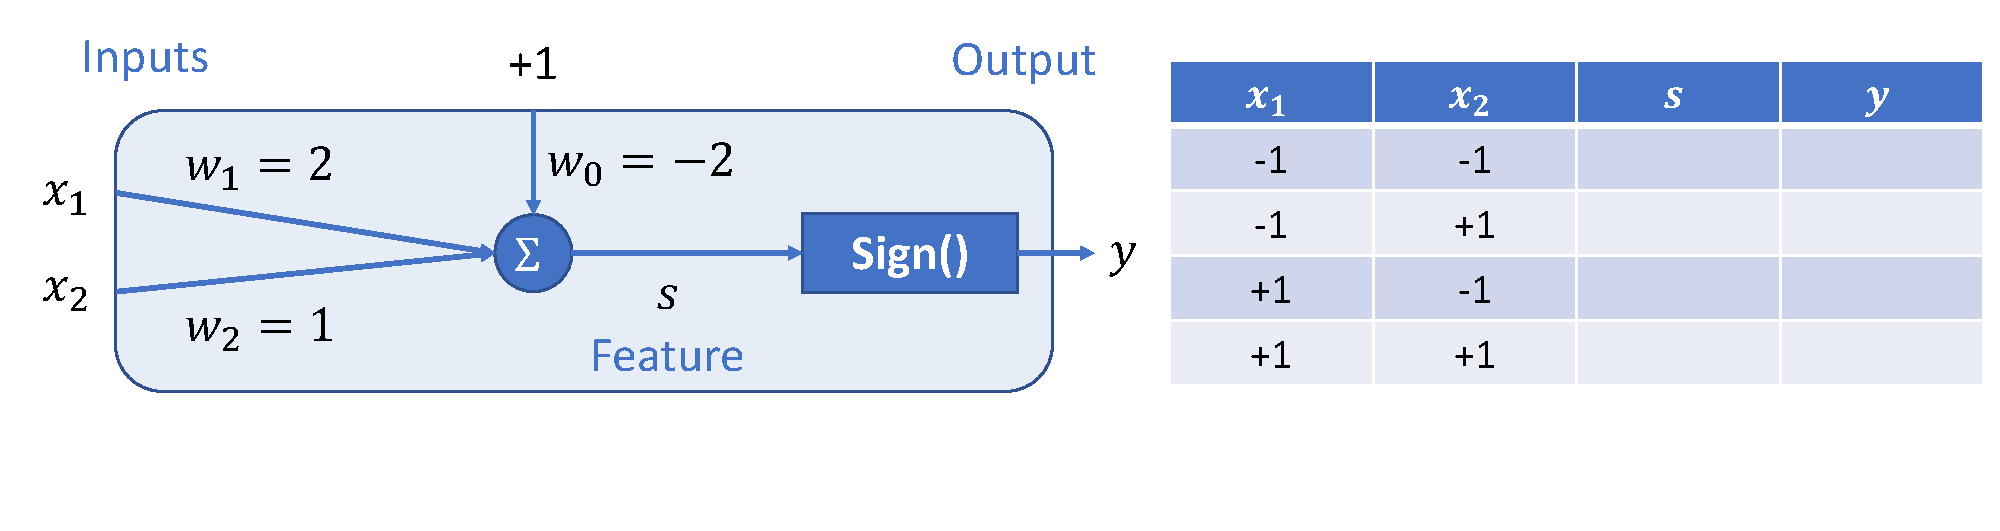
\includegraphics[width=1.0\linewidth]{Figures1.pdf}
  \vspace{-10pt}
  \caption{Problem 2.1.}
  \label{fig:2.1}
  \vspace{-10pt}
\end{figure}

\paragraph{Problem 2.2 (4 pts)} Propose proper values for weight $w_0, w_1$ and $w_2$ in the Adaline shown in Figure~\ref{fig:2.2} to perform the functionality of a logic \textbf{NOR} function. Fill in the feature $s$ for each pair of inputs given in the truth table to prove the functionality is correct.

\begin{figure}[h]
\centering
  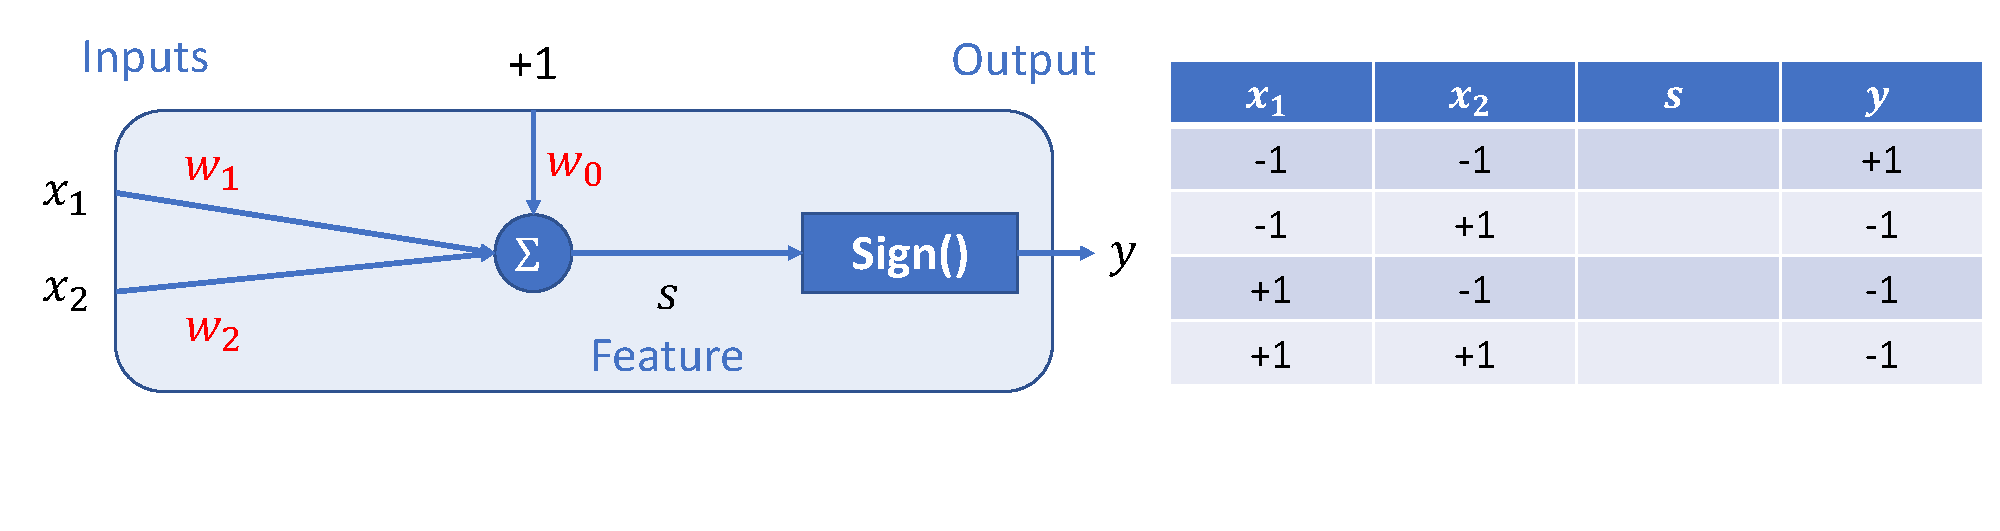
\includegraphics[width=1.0\linewidth]{Figures2.pdf}
  \vspace{-10pt}
  \caption{Problem 2.2.}
  \label{fig:2.2}
  \vspace{-10pt}
\end{figure}

\paragraph{Problem 2.3 (4 pts)} Propose proper values for weight $w_0, w_1, w_2$ and $w_3$ in the Adaline shown in Figure~\ref{fig:2.3} to perform the functionality of a \textbf{Majority Vote} function. Fill in the feature $s$ for each triplet of inputs given in the truth table to prove the functionality is correct.

\begin{figure}[h]
\centering
  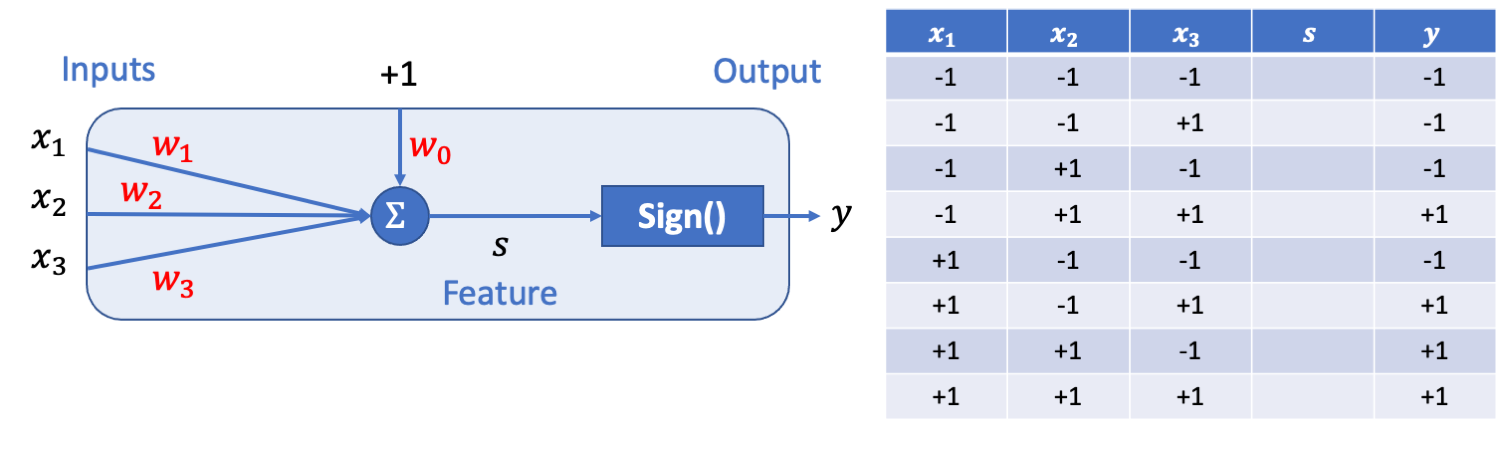
\includegraphics[width=1.0\linewidth]{Figures3.png}
  \vspace{-10pt}
  \caption{Problem 2.3.}
  \label{fig:2.3}
  \vspace{-10pt}
\end{figure}

\paragraph{Problem 2.4 (4 pts)} As discussed in Lecture 2, the XOR function cannot be represented with a single Adaline, but can be represented with a 2-layer Madaline. Propose proper values for second-layer weight $w_{20}, w_{21}$ and $w_{22}$ in the Madaline shown in Figure~\ref{fig:2.4} to perform the functionality of a \textbf{XOR} function. Fill in the feature $s$ for each pair of inputs given in the truth table to prove the functionality is correct.

\begin{figure}[h]
\centering
  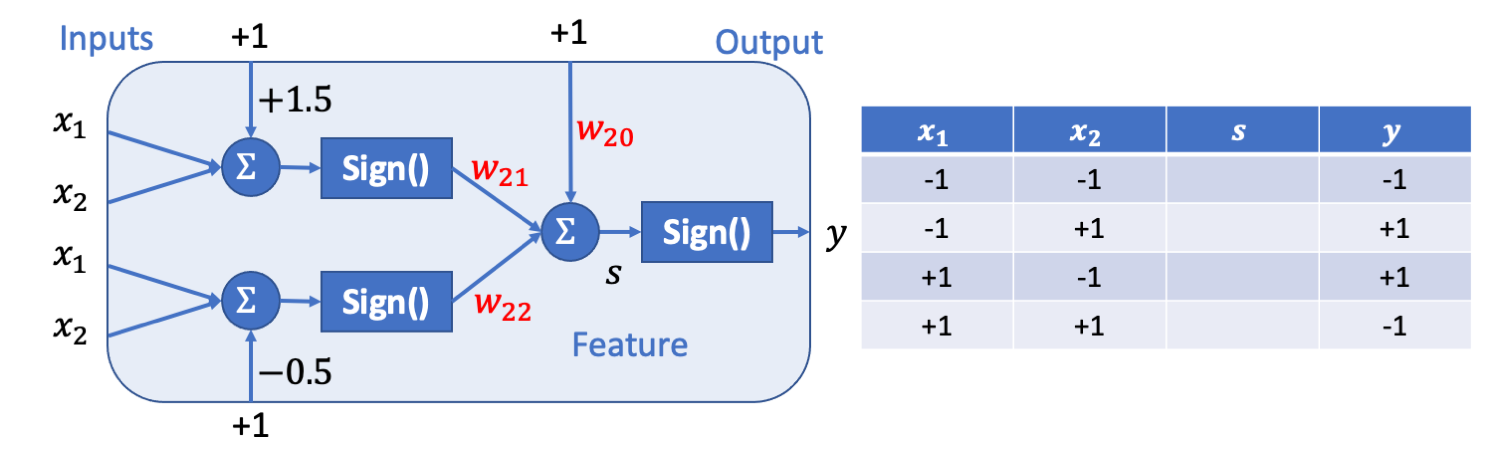
\includegraphics[width=1.0\linewidth]{Figures4.png}
  \vspace{-10pt}
  \caption{Problem 2.4.}
  \label{fig:2.4}
  \vspace{-10pt}
\end{figure}

\section{Back Propagation (10 pts)}


\paragraph{Problem 3.1 (5 pts)}
Consider a 2-layer fully-connected NN, where we have input $x_{1}\in \mathcal{R}^{n \times 1}$, hidden feature $x_{2}\in \mathcal{R}^{m \times 1}$, output $x_{3}\in \mathcal{R}^{k \times 1}$ and weights and bias $W_{1}\in \mathcal{R}^{m \times n}, W_{2}\in \mathcal{R}^{k \times m}, b_{1}\in \mathcal{R}^{m \times 1}, b_{2}\in \mathcal{R}^{k \times 1}$ of the two layers. The hidden features and outputs are computed as follows
\begin{align}
    x_{2} &= \text{ReLU}(W_{1}x_{1} + b_{1}) \\
    x_{3} &= W_{2}x_{2} + b_{2}
\end{align}
A MSE loss function $L = \frac{1}{2}(t-x_{3})^T(t-x_{3})$ is applied in the end, where $t\in \mathcal{R}^{k \times 1}$ is the target value. Following the chain rule, derive the gradient $\frac{\partial L}{\partial W_{1}}, \frac{\partial L}{\partial W_{2}}, \frac{\partial L}{\partial b_{1}}, \frac{\partial L}{\partial b_{2}}$ in a \textbf{vectorized format}.

\paragraph{Problem 3.2 (5 pts)}
Given a data $x_{1} = [0, 1 ,1]^T$, target value $t = [1, 1]^T$, weights and bias at this iteration are 
\begin{align}
    W_{1} &= \begin{bmatrix}
        2 & -1 & 1\\
        -3 & 2 & -1\\
    \end{bmatrix}, b_{1} = \begin{bmatrix}
        1 \\
        2 \\
    \end{bmatrix} \\
    W_{2} &= \begin{bmatrix}
        1 & -2\\
        -3 & 1\\
    \end{bmatrix}, b_{2} = \begin{bmatrix}
        1 \\
        1 \\
    \end{bmatrix}
\end{align}
Following the results in Problem 3.1, calculate the values of $L, \frac{\partial L}{\partial W_{1}}, \frac{\partial L}{\partial W_{2}}, \frac{\partial L}{\partial b_{1}}, \frac{\partial L}{\partial b_{2}}$

\section{2D Convolution (10 pts)}

\paragraph{Problem 4.1 (5 pts)}
Derive the 2D convolution results of the following $5\times9$ input matrix and the $3\times3$ kernel. Consider 0s are padded around the input and the stride is 1, so that the output should also have shape $5\times9$.
\begin{equation*}
    \begin{bmatrix}
    0 & 0 & 0 & 0 & 1 & 0 & 0 & 0 & 0\\
    0 & 0 & 1 & 1 & 1 & 1 & 1 & 0 & 0\\
    1 & 1 & 1 & 1 & 1 & 1 & 1 & 1 & 1\\
    0 & 0 & 1 & 1 & 1 & 1 & 1 & 0 & 0\\
    0 & 0 & 0 & 0 & 1 & 0 & 0 & 0 & 0
    \end{bmatrix} * 
    \begin{bmatrix}
    1/32 & 1/8 & 1/32 \\
    1/8 & 1/2 & 1/8\\
    1/32 & 1/8 & 1/32
    \end{bmatrix}
\end{equation*}

\paragraph{Problem 4.2 (5 pts)} Compare the output matrix and the input matrix in Problem 4.1, briefly analyze the effect of this $3\times3$ kernel on the input. (Hint: apply this kernel to an image to see the outputs)

\section{Lab: LMS Algorithm (15 pts)}

In this lab question, you will implement the LMS algorithm with NumPy to learn a linear regression model for the provided dataset. You will also be directed to analyze how the choice of learning rate in the LMS algorithm affect the final result. {\color{blue} All the codes generating the results of this lab should be gathered in one file and submit to Sakai.}

\begin{assignment}[(15 pts)]
To start with, please download the \texttt{dataset.mat} file from Sakai and load it into NumPy arrays\footnote{You may refer to \url{https://docs.scipy.org/doc/scipy/reference/generated/scipy.io.loadmat.html} for loading matrices in .mat file into NumPy arrays.}. There are two variables in the file: data $X\in\mathbb{R}^{100\times3}$ and target $D\in\mathbb{R}^{100\times1}$. Each individual pair of data and target is composed into $X$ and $D$ following the same way as discussed on Lecture 2 Page 8. Specifically, each row in $X$ correspond to the transpose of a data point, with the first element as constant 1 and the other two as the two input features $x_{1k}$ and $x_{2k}$. The goal of the learning task is finding the weight vector $W\in\mathbb{R}^{3\times1}$ for the linear model that can minimize the MSE loss, which is also formulated on Lecture 2 Page 7.

\begin{enumerate}[(a)]
\item (3pt) Directly compute the least square (Wiener) solution with the provided dataset. What is the optimal weight $W^*$? What is the MSE loss of the whole dataset when the weight is set to $W^*$?
\item (4pt) Now consider that you can only train with 1 pair of data point and target each time. In such case, the LMS algorithm should be used to find the optimal weight. Please initialize the weight vector as $W^0 = [0,0,0]^T$, and update the weight with the LMS algorithm. After each \textit{epoch} (every time you go through all the training data and loop back to the beginning), compute and record the MSE loss of the current weight on the whole dataset. Run LMS for 20 epochs with learning rate $r=0.01$, report the weight you get in the end and plot the MSE loss \textit{in log scale} vs. Epochs.
\item (3pt) Scatter plot the points $(x_{1k}, x_{2k}, d_k)$ for all 100 data-target pairs in a 3D figure\footnote{Please refer to \url{https://jakevdp.github.io/PythonDataScienceHandbook/04.12-three-dimensional-plotting.html} for plotting 3D plots with Matplotlib.}, and plot the lines corresponding to the linear models you got in (a) and (b) respectively in the same figure. Observe if the linear models fit the data well.
\item (5pt) Learning rate $r$ is an important hyperparameter for the LMS algorithm, as well as for CNN optimization. Here, try repeat the process in (b) with $r$ set to 0.005, 0.05 and 0.5 respectively. Together with the result you got in (b), plot the MSE losses of the 4 sets of experiments in log scale vs. Epochs in one figure. Then try further enlarge the learning rate to $r=1$ and observe how the MSE changes. Base on these observations, comment on how learning rate affects the speed and quality of the learning process. (Note: The learning rate tuning for the CNN optimization will be introduced in Lecture 7.)
\end{enumerate}
\end{assignment}

\section{Lab: Simple NN (40 pts)}
For getting started with deep Neural Network model easily, we consider a simple Neural Network model here and details of the model architecture is given in Table~\ref{tab:simple NN}.
This lab question focuses on building the model in PyTorch and observing the shape of each layer's input, weight and output. Please refer to the \textbf{NumPy/PyTorch Tutorial slides} on Sakai and the official documentations if you are unfamiliar with PyTorch syntax.

Please finish this lab by completing the \texttt{SimpleNN.ipynb} notebook file provided on Sakai. {\color{blue} The completed notebook file should be submitted to Sakai.}

\begin{table} [h]
    \centering
    \begin{tabular}{|c|c|c|c|c|c|}
         \hline
         Name & Type & Kernel size & depth/units & Activation & Strides\\
         \hline
         Conv 1 & Convolution & 5 & 32 & ReLU & 1 \\
         MaxPool & MaxPool & 3 & N/A & N/A & 2 \\
         Conv 2 & Convolution & 5 & 32 & ReLU & 1 \\
         MaxPool & MaxPool & 3 & N/A & N/A & 2 \\
         Conv 3 & Convolution & 5 & 64 & ReLU & 1 \\
         MaxPool & MaxPool & 3 & N/A & N/A & 2 \\
         FC1 & Fully-connected & N/A & 64 & ReLU & N/A \\
         FC2 & Fully-connected & N/A & 10 & ReLU & N/A \\
         \hline    \end{tabular}
    \caption{The padding for all three convolution layers is 2. A flatten layer is required before FC1 to reshape the feature.}
    \label{tab:simple NN}
\end{table}

\begin{assignment}[(40 points)]
In the notebook, first run through the first two code blocks, then follow the instructions in the following questions to complete each code block and acquire the answers. 

\begin{enumerate}[(a)]
\item (10pt) Complete code block 3 for defining the adapted SimpleNN model. Note that customized \texttt{CONV} and \texttt{FC} classes are provided in code block 2 to replace the nn.Conv2d and nn.Linear classes in PyTorch respectively. The usage of the customized classes are exactly the same as their PyTorch counterparts, the only difference is that in the customized class the input and output feature maps of the layer will be stored in \texttt{self.input} and \texttt{self.output} respectively after the forward pass, which will be helpful in question (b). After the code is completed, run through the block and make sure the model forward pass in the end throw no errors. Please copy your code of the completed \texttt{SimpleNN} class into the report PDF.
\item (30pt) Complete the for-loop in code block 4 to print the shape of the input feature map, output feature map and the weight tensor of the 5 convolutional and fully-connected layers when processing a single input. Then compute the number of parameters and the number of MACs in each layer with the shapes you get.
In your report, use your results to fill in the blanks in Table~\ref{tab:6b}.
\end{enumerate}

\end{assignment}

\begin{table} [h]
    \centering
    \begin{tabular}{|c|c|c|c|c|c|}
         \hline
         Layer & Input shape & Output shape & Weight shape & \# Param & \# MAC \\
         \hline
         Conv 1 &  &  &  &  &   \\
         Conv 2 &  &  &  &  &   \\
         Conv 3 &  &  &  &  &   \\
         FC1 &  &  &  &  &   \\
         FC2 &  &  &  &  &   \\
         \hline    \end{tabular}
    \caption{Results of Lab 2(b).}
    \label{tab:6b}
\end{table}


\begin{assignment}[(Bonus 10 points)]
Please first finish all the required codes in Lab 2, then proceed to code block 5 of the notebook file.

\begin{enumerate}[(a)]
\item (2pt) Complete the for-loop in code block 5 to plot the histogram of weight elements in each one of the 5 convolutional and fully-connected layers.
\item (3pt) In code block 6, complete the code for backward pass, then complete the for-loop to plot the histogram of weight elements' gradients in each one of the 5 convolutional and fully-connected layers. 
\item (5pt) In code block 7, finish the code to set all the weights to 0. Perform forward and backward pass again to get the gradients, and plot the histogram of weight elements' gradients in each one of the 5 convolutional and fully-connected layers. Comparing with the histograms you got in (b), are there any differences? Briefly analyze the cause of the difference, and comment on how will initializing CNN model with zero weights will affect the training process. (Note: The CNN initialization methods will be introduced in Lecture 6.)  
\end{enumerate}
\end{assignment}

